\section{Verklemmungen}\label{sec:deadlockreason}

\begin{tcolorbox}[enlarge top by=0.5cm,enlarge bottom by=0.5cm]
    Ein \textbf{Betriebsmittel} ist ein Objekt, auf das ein Thread unter Umständen warten muss, bevor er es benutzen kann; es kann auch ein Objekt sein, dessen Nutzung durch höchstens einen Thread zu einem Zeitpunkt über Semaphore oder Locks realisiert wird (vgl.~\cite[186]{Oec22}).
\end{tcolorbox}\\

\noindent
Folgende Bedingungen müssen erfüllt sein, damit es zu einer \textbf{Verklemmung} kommt:

\begin{enumerate}
    \item Betriebsmittel sind nur unter gegenseitigem Ausschluss nutzbar (exklusiv).
    \item Betriebsmittel, die in Verwendung sind, können dem benutzenden Thread nicht entzogen werden.
    \item Threads besitzen bereits Betriebsmittel und fordern weitere an.
    \item Folgende Bedingung gilt genau dann, wenn eine Verklemmung konkret vorliegt:
    \begin{itemize}
        \item[] Es gibt eine zyklische Kette von Threads, von denen jeder mindestens ein Betriebsmittel besitzt, das der nächste Thread in der Kette benötigt.
         \begin{figure}
            \centering
            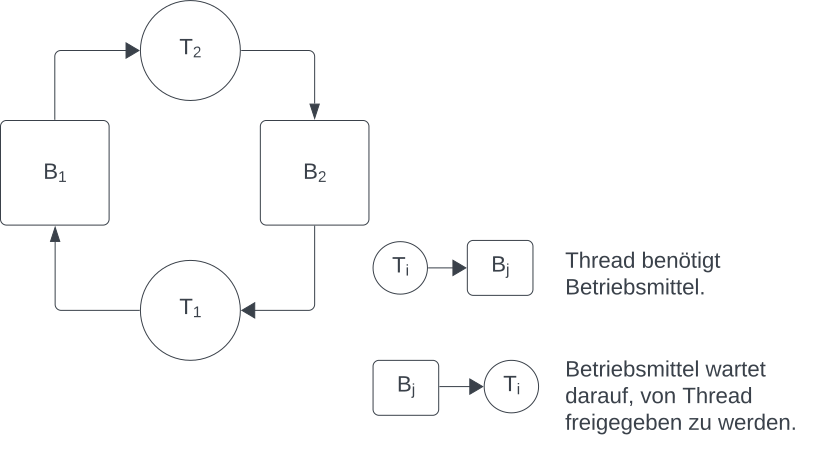
\includegraphics[scale=0.4]{chapters/fopt2/img/cyclic}
            \caption{Betriebsmittelgraph. (Quelle: in Anlehnung an \cite[192, Bild 3.9]{Oec22})}
            \label{fig:cyclic}
        \end{figure}
    \end{itemize}
\end{enumerate}


\subsection{Vermeidung von Verklemmungen}

Wenn eine der im vorherigen Abschnitt~\ref{sec:deadlockreason} genannten Bedingungen nicht gilt, kann keine Verklemmung vorliegen.\\

\noindent
In vielen Fällen ist \textbf{gegenseitiger Ausschluss} notwendig, weshalb Punkt 1 nicht abgeändert werden kann.\\

\noindent
Realisierung von \textbf{Betriebsmittelentzug} (Punkt 2) ist möglich, aber aufwändig.\\

\noindent
Gegenmaßnahmen ergeben sich aus den Bedingungen in Punkt 3 und 4\footnote{
vgl. im folgenden \cite[192 f.]{Oec22}.
}.\\

\begin{enumerate}
    \item Ein Thread darf nur Betriebsmittel anfordern, wenn er selbst keine Betriebsmittel besitzt (Nichterfüllung Punkt 3)
    \item Anforderung von Betriebsmitteln in einer bestimmten Reihenfolge, sodass garantiert werden kann, dass keine zyklischen Wartebedingungen entstehen (Nichterfüllung Punkt 4)
    \item Ein Thread $t_1$ darf auf ein Betriebsmittel, dass $t_2$ gerade benutzt, nur warten, wenn bestimmte Beziehungen zwischen $t_1$ und $t_2$ gelten, damit keine zyklischen Wartebeziehungen entstehen (Nichterfüllung Punkt 4)
    \item Eine Bedarfsanalyse untersucht bei der Anforderung von Betriebsmitteln, ob es im worst-case bei Erfüllung der Anforderung zu Verklemmungen kommen kann - wenn selbst im worst-case keine Verklemmung entstehen kann, wird die Anforderung erfüllt (Nichterfüllung Punkt 4)
\end{enumerate}\\

\noindent
Realisierung mit Hilfe eines \textbf{ResourceManagers}, der alle Betriebsmittel kennt.\\

\noindent
Threads fragen ResourceManager an, der die Betriebsmittel dann zuweist.\\

\noindent
Anfordern von Betriebsmittel auf einen Schlag (s. \textbf{Semaphorgruppe}), damit es zu keiner Verklemmung kommen kann (s. \textbf{Philosophenproblem}).\\

\noindent
Betriebsmittel gemäß einer vorgegebenen Reihenfolge anfordern, damit keine Verklemmungen entstehen können.\\
Bspw. durch Nummerierung der Betriebsmittel in \textit{aufsteigender Reihenfolge}, so dass ein Thread nur Betriebsmittel des Typs $s$ anfordern darf, wenn er keine Betriebsmittel des Typs $s$ oder $t > s$ hält\footnote{
    dann werden ihm nur Betriebsmittel vom Typ $t < s$ zugeteilt.
}).\\
Umsetzung beim Philosophenproblem: Alle Philosophen bis auf einen fordern zunächst links, dann rechts an, und einer in umgekehrter Richtung (man erhält dann immer eine verklemmungsfreie Lösung, vgl.~\cite[197]{Oec22}).\\

\noindent
Anforderung von Betriebsmitteln mit Bedarfsanalyse (\textbf{Bankier-Algorithmus}); Überprüfen der Anforderungen in Hinsicht auf sichere/unsichere Belegzustände, nur zuteilen von Betriebsmitteln, wenn sichere Belegzustände garantiert werden können.


\subsection{Zusammenfassung}
Eine \textbf{Verklemmung} ist eingetreten, wenn es einen Zyklus von Threads gibt, so dass ein Thread auf ein Betriebsmittel wartet, welches der im Zyklus folgende Thread besitzt.\\

\noindent
\textbf{Betriebsmittel}: Objekte, deren Zugriff mittels \code{synchronized}, \textbf{Semaphore} oder \textbf{Locks} synchronisiert werden.\\

\noindent
Voraussetzung für Verklemmungen sind, dass Betriebsmittel nur unter gegenseitigem Ausschluss nutzbar sind, einem Thread nicht entzogen werden können, und dass ein Thread bereits Betriebsmittel hält und weitere anfordert.\\

\noindent
Zur Vermeidung von Verklemmungen bieten sich verschiedene Strategien an, {bspw.} Anfordern der Betriebsmittel auf einen Schlag, in einer bestimmten Reihenfolge oder Durchführung einer Bedarfsanalyse vor der Zuteilung, {bspw.} mithilfe des Bankier-Algorithms.
